% !TEX TS-program = pdflatex
% !TEX encoding = UTF-8 Unicode
\documentclass[11pt]{article} % use larger type; default would be 10pt

\usepackage[utf8]{inputenc} % set input encoding (not needed with XeLaTeX)
%
%%% PAGE DIMENSIONS
\usepackage{geometry} % to change the page dimensions

\geometry{a4paper} % or letterpaper (US) or a5paper or....,
%\geometry{margin=2in} % for example, change the margins to 2 inches all round
% \geometry{landscape} % set up the page for landscape
%   read geometry.pdf for detailed page layout information 
\usepackage{caption}
\usepackage{subcaption}
\usepackage{graphicx, xcolor} % support the \includegraphics command and options
\usepackage{siunitx}
%\usepackage[parfill]{parskip} % Activate to begin paragraphs with an empty line rather than an indent

%%% PACKAGES
\usepackage{booktabs} % for much better looking tables
%\usepackage{multirow}
\usepackage{array} % for better arrays (eg matrices) in maths
\usepackage{amssymb} % for math symbols (e.g. real numbers)
%\usepackage{paralist} % very flexible & customisable lists (eg. enumerate/itemize, etc.)
%\usepackage{verbatim} % adds environment for commenting out blocks of text & for better verbatim

\usepackage{wrapfig}

\usepackage{nameref}

\usepackage{color, soul}

\usepackage[backend=bibtex,sorting=none]{biblatex}
\bibliography{bibliography.bib}

%%% SECTION TITLE APPEARANCE
% (This matches ConTeXt defaults)
\usepackage{pdfpages}
\usepackage{hyperref}
\hypersetup{
  colorlinks=true,%activates colors
  allcolors=blue,%default color
  linkcolor=blue,
  filecolor=magenta,
  urlcolor=cyan,
}
%%% END Article customizations
%
%%% The "real" document content comes below...
%
\title{Memory effect in news' spreading networks: data analysis}
\author{Nicola Sella, Francesco Fanchin}
%\date{} % Activate to display a given date or no date (if empty),
         % otherwise the current date is printed
\begin{document}
\maketitle
\begin{abstract}
  \noindent Agent-based models (ABM) have been widely applied for complex systems
  modeling.
  A set of microscopic rules define agent's autonomous and
  cooperative actions: at a macroscopic level, the overall system
  exhibits the so-called ``emergent behavior''.
  Rumor spreading in networks is a natural environment where ABM
  could explain complex phenomena like echo chambers.
  Agents' memory is not generally taken into account by ABM
  literature: we do consider it in our analysis.
  As a starting point, we will rely on our previous work,
  ``Memory effects in news' spreading networks''.\\
  We developed a network framework where agents interact with themselves.
  Network's structure and the software codes were
  formerly explained: now we will pay particular attention to
  the connection between agents' memory length  and some of the
  network's statistical properties.
  Precisely we will measure, over different memory sizes, average
  clustering coefficient, diameter of the network and Gini index
  of news' distribution.\\
  We will define a measurement procedure based on weighted
  regression; then we will suggest a phenomenological description for
  each of the measured quantities.
  In addition, a qualitative study of echo chambers phenomenon is provided.
\end{abstract}
\thispagestyle{empty}
\newpage
\thispagestyle{empty}
\tableofcontents
\listoffigures
\listoftables
\newpage
\pagenumbering{arabic}
\section{Introduction}
This paper represents natural prosecution of the previous work ''Memory effects in news' spreading networks'' by the same authors.
While the first explained network's structure and its main functionalities, this one investigates possible relationships between agents' memory and some network's statistical properties.
Precisely, we will measure, with various levels of memory, gini index of news' distribution, clustering and diameter.
After indicating a precise measurement procedure, a regression and a phenomenological description will be provided for each one of them.
\newpage

\section{Effects on the network}
All agents in our network have a fixed \textit{memory length}, i.e. they can remember a maximum
 amount of news.
In this section, its influence in network topology will be studied: clustering and
 diameter are standard measures in network science's literarure and widely used to describe
 network properties.\\
  Each of them will be plotted
 against memory length to search possible correlations.
\subsection{Clustering} \label{clustering}
A large number of networks show a tendency for link formation
between neighboring vertices, i.e., the network topology deviates
from uncorrelated random networks: this tendency is called
\textit{clustering}.\cite{clusterarticle}\\
For unweighted graphs, the clustering of a node $u$ is the fraction
of possible triangles over all possible triplets
through that node that exist,\cite{clustersite}

\begin{equation}
\label{eq:clustering}
c_u = \frac{2 T(u)}{deg(u)(deg(u)-1)}
\end{equation}
where $T(u)$ is the number of triangles through node $u$ and $deg(u)$ is the degree of $u$.
Hence, the \textit{average clustering coefficient}  is:
\begin{equation}
\label{eq:averageclustering}
ACC = \frac{1}{n}\sum_{v \in G} c_v
\end{equation}
We ask wether memory, previously considered in section
\ref{introduction}, could affect the average clustering coefficient.
To answer the question, the following experiment was designed:
for every memory size, five simulations were run over a thousand
iterations; $ACC$'s mean and standard deviation were computed
afterwards.\\
Finally, via weighted interpolation, a plot of $ACC$'s mean
over memory size will show possible  correlations.
Results and discussion are reported in section \nameref{diameter}.
\begin{figure}[h]
  \centering
  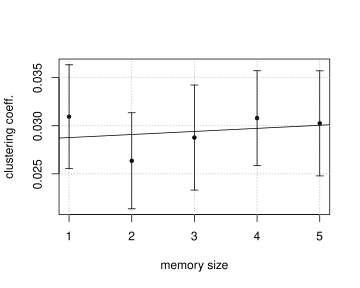
\includegraphics[trim={0cm 0cm 0cm 1cm},clip,width=.8\columnwidth]{img/clustering.pdf}
  \caption{ACC's mean-memory size linear weighted fit: five simulations per point.\label{fig:clustering}}
\end{figure}

\subsection{Diameter} \label{diameter}
In graph theory, \textit{shortest path}\cite{diameter} (SP)
between node $a$ and $b$ of a graph is the minimum number of
edges connecting them (i.e. the minimum number of ``steps'' to go
from $a$ to $b$).\\
After computing SP for every couple of nodes in a graph, we can
define \textit{diameter}\cite{diameter} as the maximum of the
shortest paths.\\
As with clustering, we ran five  simulations for every memory
size, obtaining a plot of diameter's mean over memory size with
errors. Final regression will point out possible correlations.
\begin{figure}[h]
  \centering
  \includegraphics[trim={0cm 0cm 0cm 1cm},clip,width=.8\columnwidth]{img/diameter.pdf}
  \caption{diameter's mean-memory size linear weighted fit: five simulations per point.}
  \label{fig:diameter}
\end{figure}
\begin{table}[h]
\label{tab:clusteringdiameter}
\centering
\begin{tabular}{r|cccc}
\toprule
& Slope & Intercept & $R^2$ & $\rho_{xy}$ \\
\midrule
\textit{Clustering} & $(3 \pm 6) \cdot 10^{-4}$ &$(2.8 \pm 0.2) \cdot 10^{-2}$ &$6.8 \cdot 10^{-2}$ & $2.5 \cdot 10^{-1}$ \\
\textit{Diameter} & $(0.3 \pm 1.2) \cdot 10^{-1}$ & $8.2 \pm 0.4$ & $1.8 \cdot 10^{-2}$ & $1.8 \cdot 10^{-1}$  \\
\bottomrule
\end{tabular}
\caption{Fitting results for clustering and diameter.}
\end{table}
We can visually notice that both measures are weakly correlated with
memory length: low values of correlation indexes
$\rho_{xy}$ give us a confirmation.\\
$R^2s$ are close to zero too: the reason lies in the  formula
of $R^2$.\footnote{Let us suppose to have N datapoints
$(x_i,y_i)$ and $f_i$ be the
value of fitting function in the x-axis.Coefficent of determination
$R^2s$ is: $R^{2}= 1-{\frac {SS_{ res}}  {SS_{ tot}}}$
with:
$SS_{ res}=\sum_{i=1}^{i=N}{(y_i - f_i)^2}$
and
$SS_{ tot}=\sum_{i=1}^{i=N}{(y_i - \bar{y})^2}$
As slope of the fitting function tends to zero, $SS_{res}$ tends
to $SS_{tot}$: in the limit case, if $f$ is a constant function,
$f_i=k$ $\forall  i$,  $k \in  \mathbb{R}$ and the least
squares function becomes: $E(k)= \sum_{i=1}^{N}{(k-y_i)^2} $
Setting the first derivative of $E(k)$ to zero, it can easily proved
that minimum of $E(k)$ is reached for $k=\bar{y}$.}
Hence, the fraction gets closer to one and $R^2$ tends to zero.


\newpage
\section{Effects on Users} \label{sec:users}
Memory selects the amount of news can be remembered: this could
affect news' distribution among users.
Indeed, if we insert in the network a certain number of news
(i.e. launching a simulation with many news), they will reach a
fraction of users (\textit{FOUR}, fraction of users reached)
at a fixed time.\\
News spreading over time, in general, starts with a fluctuating
transient and then reaches a stationary state: from a ``microscopic''
point of view, users' identity might vary but the fraction is
pretty much the same. \\
It is statistically correct to compute, for every news, the average
\textit{FOUR} over time, with a certain threshold in order to
neglect the transient (the end time and the threshold are
experimentally determined by free trials).
We obtain in this  way a distribution of average \textit{FOURs},
one for each news.\\
\subsection{Gini Index}
\textit{Gini index}\cite{ginindex} measures the inequality of a
distribution. Values of 0 and 1 stand for, respectively, the
maximum homogeneity and the maximum heterogeneity.
However, this index is a function of random values: mean and
error have to be estimated.\\
A certain number of samples is created by sampling with replacement
of the average FOUR distribution: Gini index is computed for each
one of them.
Now we have a population of Gini indexes, and we can extract
mean and error: the whole process is known as
\textit{bootstrap}\cite{bootstrap}
(see \hl{Appendix 1} for error estimation).\\
In practical terms, for every level of  memory, a simulation with
twenty news is run out: Gini index' mean and error are computed
like before.
The Gini index-memory plot shows a highly non-linear behaviour:
sigmoid and gaussian seem to better represent data.\\
In order to select the best-fit function, \textit{Chi-square} is
computed for both of them. \\
Because of asymmetric error bars, the optimization function is
slightly different from the standard one, used for weighted
interpolation: see \hl{Appendix 2} for more details.
Interpolation results are shown below:

%\begin{figure}[!h]
  %\centering
  %\includegraphics[width=.7\columnwidth]{img/gini_memory.png}
  %\caption{Gini index-memory plot with errorbars}
  %\label{fig:ginimem}
%\end{figure}




\begin{figure}[h]
  \centering
  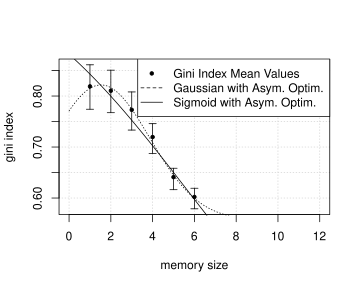
\includegraphics[trim={0cm 0cm 0cm 1cm},clip,width=.8\columnwidth]{img/gini.pdf}
  \caption{Gini index on memory size.}
  \label{fig:gini}
\end{figure}

\begin{table}[h]
  \centering
  \begin{tabular}{rSSSS}
    \toprule
    & \multicolumn{2}{c}{\textit{Gaussian Fit}} & \multicolumn{2}{c}{\textit{Sigmoid Fit}}\\
     & {$\chi^2$} & {p-value} & {$\chi^2$} & {p-value} \\ \midrule
    stde & 0.0013260 & 0.97195 & 0.00080793 & 0.97732 \\
    qant & 0.0037563 & 0.95113 & 0.0012997  & 0.97124 \\
    asym & 0.0013576 & 0.97061 & 0.00084281 & 0.97684 \\ \bottomrule
  \end{tabular}
  \caption{Reduced $\chi^2$ and respective p-value for Gaussian
    and Sigmoid fit with different non-linear optimization
    strategies.\\
    Optimization using the standard error of the Gini index
    is denoted as std, quantile bootstrap optimization\cite{quantile} as
    quant and asymmetric error bar fitting optimization as asym.}
  \label{tab:gini}
\end{table}

We can notice that, for every type of errorbar, sigmoid's
$\chi^2$ is slightly lower than gaussian one; p-value is
higher instead.
Null hypothesis, for both measures, is far from being rejected:
goodness-of-fit is solidly validated.
Hence, sigmoid is our best-fit function for gini index-memory
length plot.

\subsection{Echo chambers}
In news media, \textit{echo chamber} is a metaphorical description
of a situation in which beliefs are amplified or reinforced by
communication and repetition inside a closed system\cite{echochamwiki,echocham}.\\
We qualitatively investigated the presence of echo chambers in our network.
First of all, our agents have a ``mental  state'', i.e. a vector of preferences: its components represent the amount of interest toward a certain topic.\\
 News have the same dimension of \textit{mental state vector} (MSVD) in order to establish a ``matching'' between news' topics and users' preferences.
 Mental state is highly involved in news' dynamics and network topology.\footnote{See section~\ref{introduction} for more details on the previous work.}\\
 In the images below, for MSVD=3,5,7, we extracted main clusters from our network.
 Memory length is twelve for all the simulations.\\
 \textit{Modularity} is a measure for detecting community structure in graphs\cite{modulwiki}.
 To provide a comparison, nodes were painted with modularity class and the most recent news in memory.
 In case of news' homogeneity inside a single cluster, we are observing an echo chamber.\\
We can notice that number of clusters equals MSVD basically.
News' situation is more heterogenous: altough some clusters still exist, there is not a clear separation among users with different news.


\begin{figure}

  \centering
  \begin{subfigure}[t]{0.25\textwidth}
    \includegraphics[width=\textwidth]{img/dim3_mod.pdf}
    \label{fig:bubble3mod}
    \caption{}
  \end{subfigure}
  ~
  \begin{subfigure}[t]{0.35\textwidth}
    \includegraphics[width=\textwidth]{img/dim5_mod.pdf}
    \label{fig:bubble5mod}
    \caption{bubble3news}
  \end{subfigure}
  ~
  \begin{subfigure}[t]{0.35\textwidth}
    \includegraphics[width=\textwidth]{img/dim7_mod.pdf}
    \label{fig:bubble7mod}
    \caption{bubble3news}
  \end{subfigure}
  \\
  \begin{subfigure}[t]{0.25\textwidth}
    \includegraphics[width=\textwidth]{img/dim3_news.pdf}
    \label{fig:bubble3news}
    \caption{bubble3mod}
  \end{subfigure}
  ~
  \begin{subfigure}[t]{0.35\textwidth}
    \includegraphics[width=\textwidth]{img/dim5_news.pdf}
    \label{fig:bubble5news}
    \caption{bubble3news}
  \end{subfigure}
  ~
  \begin{subfigure}[t]{0.35\textwidth}
    \includegraphics[width=\textwidth]{img/dim7_news.pdf}
    \label{fig:bubble5news}
    \caption{bubble3news}
  \end{subfigure}
  \caption{Simulations for 1000 users and 20 sources after 1000
    iterations. (\ref{fig:bubble3mod}), (\ref{fig:bubble5mod}) and
    (\ref{fig:bubble7mod}) highlights state vector.
    (\ref{fig:bubble3news}), (\ref{fig:bubble3news}) and
    (\ref{fig:bubble3news}) hightlitghts different news.
}
  \label{fig:test}
\end{figure}

\newpage
\section{Conclusion and further developments}
This paper has shown a correlation between memory length and Gini
index of news' distribution: a suitable optimization function
was developed in order to properly fit experimental data.
With reference to network topology, memory does not significantly
affect clustering and diameter.
There is not, at the moment, a clear evidence of echo chambers.\\
\\
Further developments include longer simulations with more nodes:
the overall system is not generally scale-invariant.
Hence, we expect different behaviors (like a more
distinct observation
of echo chambers) at higher orders of magnitude.\\
In addition, other agents' actions or news' features could be added for a better realism.
For example, news are characterized by a certain amount of different topics.\\
However, they are not perceived as bad or good by agents: this additional ``degree of freedom''
could be inserted in the algorithm.

\newpage
\appendix
\section{Errorbars for Gini index}\label{Appendix A}

\textit{Bootstrap} method\cite{bootstrap} is used to compute
\textit{Gini index}' mean and error: while for the former the process
is pretty straigthforward, this is not the case for the latter.
The average fraction of users reached distribution is asymmetrical and, in general,
non-normal; we consider two different types of error.
Given N samples ${x_1,...,x_N}$ whose mean is $\mu$,
\textit{correct standard deviation} is:
$\sigma=\sqrt{\frac{\sum_{i=1}^{i=N}(x_i - \mu)^2}{N-1}}$.\\
\textit{Quantile Standard Error}\cite{quantile} (QSE), instead,
estimates the error by considering the fraction of samples
falling within a certain interval: the whole distribution is
divided in equal parts by a certain amount of ``quantiles''.\\
For example, in a Normal distribution, the interval
$[\mu -\sigma, \mu +\sigma]$ ``covers'' approximately $68\%$
of the samples.
In ``quantiles'' terms (percentiles in this case), our errorbar
starts from the $17^{th}$ percentile and ends in the $68^{th}$
percentile.\\
For non-normal distributions, standard deviation in general does
not follow this property: to preserve it, we can compute QSE with
the previous choice of quantiles, just by looking at the cumulative
distribution, when values 0.17 and 0.68 are reached.
\begin{table}[htpb]
  \centering
  \begin{tabular}{rc|cc}
    \toprule
    \multicolumn{2}{c}{\textit{quantile}} & $16\%$ & $84\%$ \\
    \midrule
    Number & \SI{10}{} & \SI{1.3e-2}{}  & \SI{8.57e-3}{} \\
    of & \SI{e3}{} & \SI{2.39e-2}{} & \SI{5.64e-3}{} \\
    boot & \SI{e5}{} & \SI{2.36e-2}{} & \SI{5.22e-3}{} \\
    samples & \SI{e7}{} & \SI{2.36e-2}{} & \SI{5.34e-3}{} \\
    \bottomrule
  \end{tabular}
  \caption{Quantile errors.}
  \label{tab:quantile}
\end{table}
\begin{figure}[h!]
  \centering
  \includegraphics[width=.8\columnwidth]{img/bootstrap.pdf}
  \caption{Several bootstraps with different size are performed. Average Gini Index is computed.}
  \label{fig:bootstrap}
\end{figure}
\begin{figure}[h!]
  \centering
  \includegraphics[width=.8\columnwidth]{img/appendix.pdf}
  \caption{Three different regressions are shown for gini index-memory length plot: with standard deviation, quantiles and asymmetric errorbars.}
  \label{fig:gausssigma}
\end{figure}
The overall error is divided twofold, ``rightmost'' and ``leftmost''
the mean. For every part of the interval, we pick the ``largest''
between standard deviation and QSE, see figure (\ref{fig:gausssigma}): this conservative approach avoids
underestimations in both directions.

\section{Asymmetric errorbars fitting}\label{Appendix B}
The aim of a standard fitting problem is to find a function which
reproduces experimental observations.
Let $f_{\theta}$ be the candidate function:
$\theta=(\theta_1,...,\theta_m)$ is a vector of $m$ parameters which
completely determine function's values.
The optimization is performed with respect to $\theta$ parameters.\\
Given N datapoints with coordinates ${(x_i,y_i)}$ and y-errorbars
$\sigma_i$, $i$=1,...,N, the usual optimization function for
\textit{weighted interpolation}\cite{interpolation} is:
$$
E(\theta)= \sum_{i=1}^{N} \frac{(f_{\theta}(x_i)-y_i)^2}{\sigma_{i}^2}
$$
However, this formula is only applicable for gaussian errors,
expressed by the standard deviation: in the problem we are facing,
errorbars are not even symmetric.
We have developed an approximate optimization function which counts
in this asymmetry.
In a weighted interpolation, the weight is the square inverse of the
standard deviation: the ``shortest'' the errorbar, the closest will
be $f(x_i)$ to $y_i$.
It might be an idea to split the error in two contributions,
to be ``activated'' if the function value is greater or lower
than the experimental value.
Let a and b be, respectively, the upper and lower portion of errorbars
compared to the mean point:
the optimization function for \textit{asymmetric
  errobars interpolation} is:
$$ E= \sum_{i=1}^{N} \frac{(f(x_i)-y_i)^2}{a^{2}\mathcal{H}(f(x_i)-y_i)+b^{2}\mathcal{H}(y_i-f(x_i))} $$
$\mathcal{H}(x)$ is the \textit{Heaviside function},
$$\mathcal{H}(x):=\frac{\mathrm{d}}{\mathrm{d}x}\mathrm{max}
\{x,0\}:=\int_{-\infty}^x \delta (s) \mathrm{d}s$$ whose value
is zero for negative argument and one for positive argument.\\
The optimization is performed by an R implementation\cite{Roptim}
of \textit{Nelder-Mead algorithm},\cite{neldermeadoriginal}
also known as \textit{downhill simplex method} or
\textit{amoeba}.\cite{neldermeadnumrec}\\
This algorithm is particularly appropriate for non-linear
optimization with many local minima.
\begin{figure}[h!]
  \centering
  \includegraphics[width=.4\columnwidth]{img/err.pdf}
  \caption{Asymmetric errorbars.}
  \label{fig:errors}
\end{figure}

\newpage
\printbibliography
\end{document}